\section{Methodology}
% \addcontentsline{toc}{section}{Methodology}
\fancyhead[R]{Methodology}

\subsection{Data Collection}
\label{sec:Data Collection}

Data collection is a crucial step in model building, as the quality and relevance of the data directly impact the model’s performance.. The data for this thesis was collected from UniProt, a comprehensive resource that provides detailed protein sequence and functional information. UniProt or Universal Protein Resource is a central protein sequence, and annotation database. It is widely accepted as comprehensive and provides high-quality data, which makes it a must to perform bioinformatics and computational biology. UniProt pools in much valuable information: experimental findings, different kinds of analyses, and literature information and hence provides rich and reliable sources of further research. Researchers can receive high-quality reviewed entries with 3D structural data and catalytic properties in place, which makes the data reliable and applicable for predicting enzyme functions. \autocite{uniprotconsortiumUniProtUniversalProtein2021}

Some of the main features of UniProt are:

\begin{enumerate}
    \item Comprehensive Protein Data: UniProt contains a vast collection of protein sequences, functional annotations, and cross-references to other databases, making it a valuable resource for protein research.
    \item Reviewed Entries: UniProt contains both reviewed (Swiss-Prot) and unreviewed (TrEMBL) entries. Reviewed entries are manually curated by experts, ensuring high accuracy and reliability.
    \item Functional Annotations: Each protein entry includes detailed functional annotations, such as catalytic activity, biological processes, and involvement in pathways.
    \item 3D Structural Data: UniProt links to structural databases like PDB, providing access to 3D structures of proteins, which are crucial for understanding enzyme mechanisms.
    \item Cross-references: Extensive cross-references to other databases (e.g., PDB, BRENDA, Reactome) enhance the richness of the data.
\end{enumerate}

For this study, UniProt was chosen due to its high-quality data, extensive coverage of protein information, and user-friendly interface. The data collection process involved querying UniProt for enzyme entries with 3D structural data and catalytic activity annotations, extracting relevant information, and preprocessing the data for model development. The data retrieval process utilized the UniProt REST API to download protein data that met specific criteria. The criteria included reviewed entries with both 3D structural data and catalytic properties. The following figure illustrates the data collection process:

\begin{figure}[hbt]
    \centering
    \begin{minipage}[t]{.8\textwidth}
    \caption{Data Collection \& P2Rank Process}
    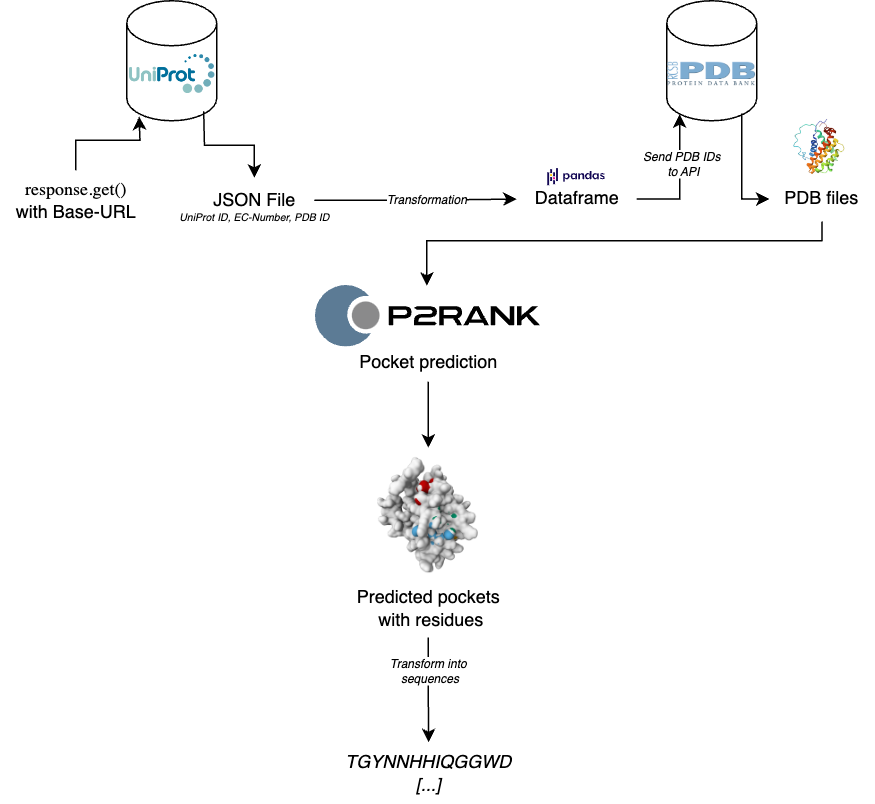
\includegraphics[width=1\textwidth]{img/Data-Preparation-Processing-Workflow.png}
    \source{Own illustration}
    \label{fig:Data-Preparation-Processing-Workflow}
    \end{minipage}
\end{figure}


\begin{compactenum}
    \item API Request: The script constructs a query to the UniProt REST API to retrieve reviewed protein entries with specified fields and criteria.
    \item Data Retrieval: Data is retrieved and transformed into a pandas DataFrame for further processing.
    \item Data Filtering: The DataFrame is filtered to retain entries with non-null EC numbers and PDB codes.
    \item PDB Download: The PDB files corresponding to the protein entries are downloaded from the PDB database using the PDB IDs.
    \item P2Rank Prediction: The P2Rank workflow is applied to the PDB files to predict interactive site residues.
    \item Data Integration: The interactive site predictions are integrated with the protein sequences for further analysis.
\end{compactenum}

\subsection{Data Preprocessing}
\label{sec:Data Preprocessing}

After data collection, the next step is to preprocess the data to make it suitable for model training. Data preprocessing involves several critical steps to prepare the dataset for the prediction model. These steps include data retrieval, cleaning, transformation, integration, and normalization. The goal of data preprocessing is to ensure that the data is clean, consistent, and suitable for training the model.

After collecting the sequences for every enzyme based on the Ligand-Binding-Site prediction, the sequences are cleaned by removing any non-standard amino acids, special characters, or gaps. \autocite{OneletterNotationAmino1972} This step ensures that the sequences contain only valid amino acid residues, which is crucial for accurate modeling.

The cleaned sequences are then tokenized and encoded into numerical data for input into the model. This involves converting each amino acid into a unique integer identifier. The sequences are also padded to ensure they all have the same length, which is necessary for batch processing in Deep Learning models. Tokenization and padding allow the model to handle sequences of varying lengths and ensure uniform input size for the neural network. \autocite{dangRepeatedPaddingData2024}

For gaining a first insight into the dataset, the distribution of EC classes in the dataset was analyzed. The table indicates that the dataset is highly imbalanced, with Transferases being the most common class and Ligases the least common. This imbalance can affect the model's performance, as it may struggle to learn from underrepresented classes. To address this issue, the dataset was balanced using the RandomUnderSampler algorithm from the imbalanced-learn library.

\begin{table}[hbt]
    \centering
    \begin{tabular}{lrr}
        \toprule
        EC Class & Count \\
        \midrule
        Oxidoreductases & 23544 \\
        Transferases & 59022 \\
        Hydrolases & 41283 \\
        Lyases & 2376 \\
        Isomerases & 4617 \\
        Ligases & 1323 \\
        Translocases & 1836 \\
        \bottomrule
    \end{tabular}
    \caption{Distribution of EC classes in the dataset}
    \label{tab:ec-class-distribution}
\end{table}

Taking a closer look at the distribution of EC classes on the second level of the hierarchy, the class 2.7 (Phosphotransferases) is the most common, while the class 2.6 (Acyltransferases) is the least common. This is because Phosphotransferases are involved in a wide range of cellular processes, making them more prevalent in the dataset. The class 2.6, on the other hand, is more specialized and less common in the dataset. After rebalancing the dataset, the distribution of EC classes is more uniform, but still not perfectly balanced. Further optimization may be required, but is beyond the scope of this study and would require additional data in the UniProt database.

Finally, the transformed features are integrated into a single dataset. The data is then normalized to ensure that all features are on a similar scale, which is important for the convergence of deep learning models. Normalization helps in speeding up the training process and achieving better performance. \autocite{ioffeBatchNormalizationAccelerating2015}

\subsection{Feature Engineering}
\label{sec:Feature Engineering}

Feature engineering is a critical step in preparing data for prediction models. This process involves transforming raw data into meaningful features that can improve the performance of the model. In this section, the author describes the feature engineering techniques used in this study, focusing on the processing of protein sequences and the calculation of additional features to enhance the predictive power of the Deep Learning model.

To capture meaningful information from protein sequences, this study used several features derived from the sequences, including amino acid composition, molecular weight, isoelectric point, hydrophobicity, and sequence length. These features provide valuable insights into the physicochemical properties of the proteins, enabling the model to learn patterns that correlate with enzyme functions. The ProteinAnalysis class ferom the Biopython library was used to calculate these features. The following Python code snippet demonstrates the calculation of additional features from the protein sequences:


The first step is to clean the protein sequence shown in chapter \ref{sec:Data Collection}. The sequence itself is used as a feature, and additional features are calculated using the ProteinAnalysis class from Biopython. To convert the cleaned sequences into a format suitable for the model, a tokenizer is used to encode the sequences into numerical data. In the context of protein sequences, each amino acid is mapped to a unique integer. For example, the sequence "ACDEFGHIKLMNPQRSTVWY" is tokenized into a list of integers. 

Tokenization involves converting each amino acid into an integer based on its position in a predefined list of valid amino acids. This process can be mathematically represented as:

\begin{align*}
    token(x)=i\quad\text{where}\quad x \in \{A, C, D, E, F, G, H, I, K, L, M, N, P, Q, R, S, T, V, \\
    W, Y\} \quad \text{and} \quad i \quad \text{is the index of amino acid} \quad x \quad \text{in the list}
\end{align*}

The tokenized sequence is then passed through an embedding layer that transforms these integers into dense vectors. This embedding process is essential for capturing the contextual meaning of each amino acid within the sequence:
$embedding(i) = v$ where $v_i$ is the embedding vector for the token $i$.
These embeddings are fed into the RNN, which processes the sequence and updates its hidden states accordingly, allowing the model to capture complex dependencies and interactions between amino acids. The sequences are then padded to ensure they all have the same length, which is necessary for batch processing in Deep Learning models.

Recent advancements have demonstrated that sequence-based models, including language models like ESM-1b, can achieve high accuracy in predicting protein functions and properties. For instance, the study by Hu et al. (2022) highlights the potential of protein-sequence based models like ESM-1b in predicting protein function from sequences. \autocite{huExploringEvolutionbasedFree2022}

In addition to tokenizing the protein sequences, several biochemical features are calculated to provide a comprehensive representation of the proteins. These features include amino acid composition, molecular weight, isoelectric point, hydrophobicity, and sequence length. The Python code for calculating these features is as follows:

\begin{enumerate}
    \item \textbf{Amino Acid Composition}: The amino acid composition represents the relative frequency of each of the 20 standard amino acids in a protein sequence.
    \begin{enumerate}
        \item Calculation: It is calculated as the percentage of each amino acid in the sequence.
        \item Relevance: Different proteins have characteristic amino acid compositions that can provide clues about their function and stability. For example, membrane proteins often have higher hydrophobic amino acid content.
        \item Example: A protein with a high proportion of hydrophobic amino acids might be involved in membrane-related processes.
    \end{enumerate}
    \item \textbf{Molecular Weight}: Molecular weight is the total mass of all amino acids in the protein sequence.
    \begin{enumerate}
        \item Calculation: It is calculated by summing the average atomic masses of the amino acids in the sequence.
        \item Relevance: The molecular weight of a protein can influence its physical and chemical properties, such as solubility and interaction with other molecules.
        \item Example: Enzymes with larger molecular weights may have multiple domains or subunits.
    \end{enumerate}
    \item \textbf{Isoelectric Point}: The isoelectric point is the pH at which the protein carries no net electrical charge.
    \begin{enumerate}
        \item Calculation: It is determined by calculating the pH at which the positive and negative charges on the amino acids balance out.
        \item Relevance: The pI affects protein solubility and interaction with other molecules. Proteins are least soluble at their pI and more likely to precipitate.
        \item Example: Proteins with a low pI are often found in acidic environments, such as lysosomal enzymes.
    \end{enumerate}
    \item \textbf{Hydrophobicity (GRAVY Score)}: The GRAVY (Grand Average of Hydropathicity) score is a measure of the overall hydrophobic or hydrophilic nature of a protein.
    \begin{enumerate}
        \item Calculation: It is calculated by averaging the hydropathy values of all amino acids in the sequence.
        \item Relevance: Hydrophobicity influences protein folding, stability, and interaction with membranes.
        \item Example: Transmembrane proteins typically have a high GRAVY score due to their hydrophobic transmembrane regions.
    \end{enumerate}
    \item \textbf{Sequence length}: The sequence length is the total number of amino acids in the protein sequence.
    \begin{enumerate}
        \item Calculation: It is simply the count of amino acids in the sequence.
        \item Relevance: The length of a protein can indicate its complexity and the number of functional domains.
        \item Example: Longer proteins may have multiple functional domains or be involved in complex regulatory mechanisms.
    \end{enumerate}
\end{enumerate}

These biochemical features provide a multi-dimensional representation of protein sequences, capturing both sequence-specific information and physicochemical properties. This feature-set is essential for analyzing the enzymes and predicting their functions accurately. A study by Gainza et al. (2020) demonstrates the importance of incorporating physicochemical features in protein function prediction models, showing that these features enhance the model's performance. For example, the choice of features such as molecular weight and isoelectric point is grounded in their proven relevance to protein function prediction. \autocite{gainzaDecipheringInteractionFingerprints2020}
\subsection{Model Development}
\label{sec:Model Development}

In this section, this studys describes the model development process, including data splitting, model architecture, and the rationale behind the chosen methods. The goal is to predict EC classes based on protein sequences using a deep learning approach enhanced by additional biochemical features.

To use diffrent models for each hierachy level, the data is split into four levels of the EC hierachy. The first level represents the broadest classification, while the fourth level provides the most specific classification. This ensures that models are trained and evaluated on appropriately structured data, allowing for predictions at varying levels of specificity.

The model architecture combines sequence-based features with additional biochemical features to enhance prediction accuracy. The architecture consists of an embedding layer, two LSTM layers, and dense layers that integrate additional features.

The embdding layer converts amino acid sequences into dense vector representations, capturing semantic similarities between amino acids. This layer allows the model to handle varying sequence lengths and to learn useful representations of amino acids in the context of their sequence. After that Long Short-Term Memory (LSTM) layers are used to capture long-range dependencies in the sequence data, which is crucial for understanding the functional context of amino acids within the sequence. LSTMs are particularly effective in modeling sequential data due to their ability to remember information for long periods and manage the vanishing gradient problem. LSTMs are particularly well-suited for tasks involving sequence data due to their ability to manage long-term dependencies and their robustness against the vanishing gradient problem. Studies have demonstrated the effectiveness of LSTMs in various sequence analysis tasks, including protein function prediction and other bioinformatics applications.\autocite{liuAttentionMechanismEnhanced2019} \autocite{zhangEncoderdecoderModelsSequencetosequence2023}

Biochemical properties such as molecular weight, isoelectric point, hydrophobicity, and sequence length are included to provide additional context that can enhance the prediction accuracy. These features help the model understand the physical and chemical characteristics of the proteins, which are critical for predicting enzyme functions. The concatenation layer combines the output of the LSTM layers with the additional biochemical features, allowing the model to leverage both sequence-based and property-based information. This integration ensures that the model considers both the sequence context and the biochemical properties of the proteins. Finally the dense layers are used to integrate the combined features and produce the final classification output. These layers apply non-linear transformations to the combined features, enabling the model to learn complex patterns and relationships.
This model uses an Adam optimizer with a learning rate of 0.001 and sparse categorical cross-entropy loss function, which is suitable for multi-class classification tasks. The model is compiled with the specified optimizer, loss function, and evaluation metrics to prepare it for training.